\documentclass[12pt]{article}
% Эта строка — комментарий, она не будет показана в выходном файле
\usepackage{ucs}
\usepackage[warn]{mathtext}
\usepackage[utf8x]{inputenc} % Включаем поддержку UTF8
\usepackage[russian]{babel}  % Включаем пакет для поддержки русского языка
\usepackage{amsmath}
\usepackage{mathtools}
\usepackage{amssymb}
% \usepackage[dvips]{graphicx}
% \graphicspath{{noiseimages/}}
\usepackage[pdftex]{graphicx}


% Параметры страницы: 1см от правого края и 2см от остальных.


\hoffset=0mm
\voffset=0mm
\textwidth=180mm        % ширина текста
\oddsidemargin=-6.5mm   % левое поле 25.4 - 5.4 = 20 мм
\textheight=240mm       % высота текста 297 (A4) - 40
\topmargin=-15.4mm      % верхнее поле (10мм)
\headheight=5mm      % место для колонтитула
\headsep=5mm          % отступ после колонтитула
\footskip=8mm         % отступ до нижнего колонтитула

\begin{document}
	\author {Жарков Андрей 495}
	\title {Лабораторная работа 5.2 \\  Моделирование оптических приборов и определение их увеличения.}
    \maketitle{}
	    
    \begin{center}
    	\textbf{\large Теоретические сведения.}
    \end{center}
    
    \textbf{Увеличение астрономической зрительной трубы.} Труба Кеплера состоит из двух собирающих линз расположенных на расстоянии $f_1 + f_2$ друг от друга (см. рис). Как было выяснено, при наблюдении далёких предметов с помощью астрономической
    зрительной трубы (трубы Кеплера) глазом, аккомодированным на бесконечность, задний фокус объектива совпадает с передним фокусом окуляра.
    В этом случае труба является афокальной системой: параллельный
    пучок лучей, входящий в объектив, остаётся параллельным по выходе
    из окуляра.
    Такой ход лучей называют телескопическим.
    
    \begin{center}
    	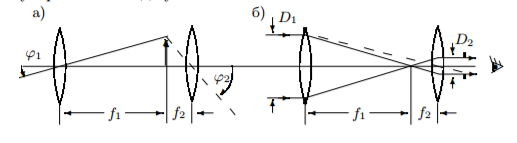
\includegraphics[width=12cm]{theory1.png}\\
    	рис. Труба Кеплера.
    \end{center}
    
    Увеличение можно найти как 
    \begin{equation}
	    \gamma = \frac{tg \varphi_2}{tg \varphi_1} = \frac{f_1}{f_2} = \frac{D_1}{D_2}
    \end{equation}
    
    \textbf{Увеличение галилеевой зрительной трубы.} Если заменить положительный окуляр астрономической трубы отрицательным, получается
    галилеева (или земная) труба. При телескопическом ходе лучей в галилеевой трубе расстояние между объективом и окуляром равно разности
    (точнее — алгебраической сумме) их фокусных расстояний (рис. 5а),
    а изображение оправы объектива, даваемое окуляром, оказываетс
    я мнимым. Это изображение располагается между объективом и окуляром.
    Легко показать, что формула (1), полученная для астрономической трубы, справедлива и для земной трубы.
    
    Достоинством галилеевой трубы является то, что она даёт прямое
    изображение. Поэтому зрительные трубы, бинокли и т.д. делаются по
    схеме Галилея.
    
    \begin{center}
    	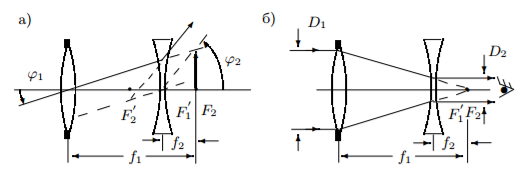
\includegraphics[width=12cm]{theory2.png}\\
    	рис. Труба Галилея
    \end{center}
    
    \textbf{Увеличение микроскопа.} Увеличение микроскопа (см. рис) можно найти, как
    
    \begin{equation}
	    \gamma = \frac{tg \varphi_2}{tg \varphi_1} = \frac{L (\Delta - f_1 - f_2)}{f_1 f_2}
    \end{equation}
    
    \begin{center}
    	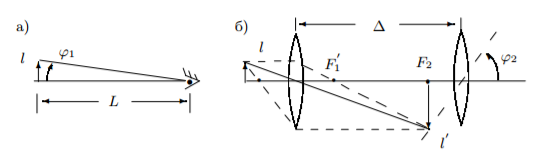
\includegraphics[width=12cm]{theory3.png}\\
    	рис. Микроскоп
    \end{center}
    
    \begin{center}
    	\textbf{\large Выполнение работы.}
    \end{center}
    
    \textbf{Измерение фокусных расстояний линз.} Настроим зрительную трубу на бесконечность. Фокусные расстояния собирающей и рассеивающей линз можно определить следующим образом:
    
    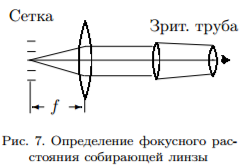
\includegraphics[width=6cm]{focus+.png}
    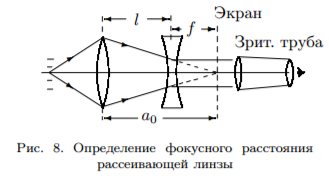
\includegraphics[width=7cm]{focus-.png}
    
    Результаты измерений в таблице ($f_{перев}$ - измерения после переворачивания линзы другой стороной, $f_{инстр}$ - по паспорту линзы)
    
    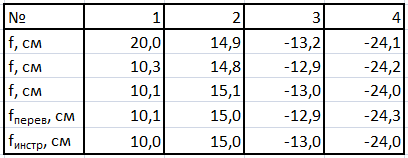
\includegraphics[width=10cm]{table1.png}
    
    Как видим, линзы можно считать тонкими. Фокусные расстояния определены с точностью до 1мм.
    
    \textbf{Труба Кеплера.}
    
    В качестве коллиматора возьмём линзу $f = 15,0 см$. Найденное $l_1 = 1,30 \pm 0,05 мм$ - размер изображения одного деления шкалы осветителя.
    
    Теперь соберём модель телескопа Кеплера ($f_1 = 40,0 sm$, $f_2 = 10,0sm$):
    
    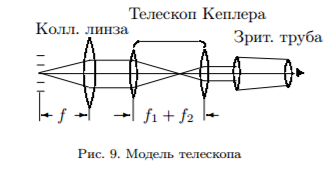
\includegraphics[width=9cm]{kepl.png}
    
    Тогда, по формуле (1) $\gamma = \frac{f_1}{f_2} = 4,00 \pm 0,04$
    
    С другой стороны, измерив $l_2 = 5,1 \pm 0,1 мм$ - размер изображения одного деления шкалы осветителя после прохождения телескопа, $\gamma = \frac{l_2}{l_1} = 3,92 \pm 0,15$
    
    Через диаметры ($D_1 = 3,2 \pm 0,1 см$, $D_2 = 0,9 \pm 0,1 см$): $\gamma = \frac{D_1}{D_2} = 3,6 \pm 0,4$
    
    В пределах погрешности найденные значения совпадают.
    
    \textbf{Труба Галилея.}
    
    В трубе $f_1 = 40,0 см$, $f_2 = -13,0см$.
    
    По формуле (1) $\gamma = \frac{f_1}{f_2} = 3,08 \pm 0,04$
    
    С другой стороны, измерив $l_2 = 4,0 \pm 0,1 мм$ - размер изображения одного деления шкалы осветителя после прохождения трубы галилея, $\gamma = \frac{l_2}{l_1} = 3,1 \pm 0,1$
    
    В пределах погрешности найденные значения совпадают.
    
    \textbf{Увеличение микроскопа.}
    
    Будем использовать линзы $f_1 = 15,0 см$, $f_2 = 10,0см$. Хочется получить $\gamma = 5$. Для этого, пользуясь (2) подберём значение $\Delta$. Получим, $\Delta = 55,0 см$. Теперь соберём установку.
    
    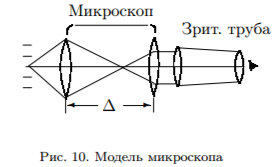
\includegraphics[width=7cm]{micro.png}
    
    Измерим $l_2 = 4,0 \pm 0,1 мм$ - размер изображения одного деления шкалы осветителя после прохождения трубы галилея. Тогда, взяв $L = 25 см$ - расстояние наилучшего зрения, можно посчитать увеличение $\gamma = \frac{l_2}{l_1}\frac{L}{f} = 5,1 \pm 0,2$.
    
    В пределах погрешности совпадает с $\gamma = 5$ - вычисленное по (2).
    
\end{document}